\documentclass[notoc, oneside, openany]{tufte-book}
\setcounter{tocdepth}{2}
\setcounter{secnumdepth}{2}

\makeatletter
% Paragraph indentation and separation for normal text
\renewcommand{\@tufte@reset@par}{%
  \setlength{\RaggedRightParindent}{0pt}%
  \setlength{\JustifyingParindent}{0pt}%
  \setlength{\parindent}{0pt}%
  \setlength{\parskip}{4pt}%
}
\@tufte@reset@par

% Paragraph indentation and separation for marginal text
\renewcommand{\@tufte@margin@par}{%
  \setlength{\RaggedRightParindent}{0pt}%
  \setlength{\JustifyingParindent}{0pt}%
  \setlength{\parindent}{0pt}%
  \setlength{\parskip}{4pt}%
}

\title{
    {\huge Appunti di}\\
    Machine Learning
}
\author{Mattia Bolognini}
\date{Ultima modifica: \today}

\makeatletter
\renewcommand{\maketitlepage}{%
\begingroup%
\setlength{\parindent}{0pt}
{\fontsize{24}{24}\selectfont\textit{\@author}\par}
\vspace{1.75in}{\fontsize{36}{54}\selectfont\@title\par}
\vspace{0.5in}{\fontsize{14}{14}\selectfont\textsf{\smallcaps{\@date}}\par}
\vfill{\fontsize{14}{14}\selectfont\textit{\@publisher}\par}
\thispagestyle{empty}
\endgroup
}
\makeatother

\geometry{
    %showframe, % for debugging purposes -- displays the margins
	left=13mm, % left margin
	textwidth=135mm, % main text block
	marginparsep=8mm, % gutter between main text block and margin notes
	marginparwidth=50mm % width of margin notes
}
\fontsize{10}{20}\selectfont

%--------Package inclusions--------
\usepackage{clrscode3e} % Pseudocode in the style of "Introduction to algorithms"
\usepackage{minted} % Code highlighting for different programming languages
\usepackage[activate={true,nocompatibility},final,tracking=true,kerning=true,spacing=true,factor=1100,stretch=10,shrink=10]{microtype}
\usepackage{pgf,tikz,tikz-cd}
\usepackage{amsmath,amsthm,amssymb,amsfonts} % Math packages
\usepackage{relsize, xfrac} % Math utilities
\usepackage{bussproofs} % Derivation tree
\usepackage{optidef} % Write optimization problem
\usepackage[italian]{babel}
\usepackage{booktabs} % Makes prettier tables.
\usepackage{multicol} % Small sections of multiple columns in documents and tables.
\usepackage{units}
\usepackage{fancyvrb} % Customization of the formatting of verbatim environments.
\fvset{fontsize=\normalsize} % Use a smaller font for the verb environment.
\usepackage{sectsty} % Customization of section commands
\allsectionsfont{\normalfont \bfseries} % All sections centered, using the default font and small caps
\usepackage{graphicx}
\setkeys{Gin}{width=\linewidth,totalheight=\textheight,keepaspectratio}
\graphicspath{/images}
\usepackage{hyperref} % Allows hyperlinks in generated PDF file
\usepackage{lipsum} % Lorem Ipsum text
\usepackage{fancyhdr} % Custom headers and footers
\pagestyle{fancyplain} % Makes all pages in the document conform to the custom headers and footers
\fancyhead{} % No page header - if you want one, create it in the same way as the footers below
\fancyfoot[L]{} % Empty left footer
\fancyfoot[C]{} % Empty center footer
\fancyfoot[R]{\thepage} % Page numbering for right footer
\renewcommand{\headrulewidth}{0pt} % Remove header underlines
\renewcommand{\footrulewidth}{0pt} % Remove footer underlines
\setlength{\headheight}{13.6pt} % Customize the height of the header
\allowdisplaybreaks

%--------Theorem Environments--------
%theoremstyle{plain} --- default
\newtheorem{thm}{Theorem}
\newtheorem{cor}[thm]{Corollary}
\newtheorem{prop}[thm]{Proposition}
\newtheorem{lem}[thm]{Lemma}
\newtheorem{conj}[thm]{Conjecture}
\newtheorem{quest}[thm]{Question}
\newtheorem{claim}{Claim}
\newtheorem{property}{Proprietà}

\theoremstyle{definition}
\newtheorem{defn}[thm]{Definition}
\newtheorem{defns}[thm]{Definitions}
\newtheorem{con}[thm]{Construction}
\newtheorem{exmp}[thm]{Example}
\newtheorem{exmps}[thm]{Examples}
\newtheorem{notn}[thm]{Notation}
\newtheorem{notns}[thm]{Notations}
\newtheorem{addm}[thm]{Addendum}
\newtheorem{exer}[thm]{Exercise}

\theoremstyle{remark}
\newtheorem{rem}[thm]{Osservazione}
\newtheorem{ans}[thm]{Answer}
\newtheorem{rems}[thm]{Remarks}
\newtheorem{warn}[thm]{Warning}
\newtheorem{sch}[thm]{Scholium}

%--------Command Definitions--------
% Operators
\newcommand{\Mod}[1]{\ (\text{mod}\ #1)}
\newcommand{\N}{\mathbb{N}}
\newcommand{\Z}{\mathbb{Z}}
\newcommand{\Q}{\mathbb{Q}}
\newcommand{\R}{\mathbb{R}}
\newcommand{\C}{\mathbb{C}}
\newcommand{\OR}{\,|\,}
\newcommand{\AND}{\,\&\,}
\newcommand{\NOT}{!}

% Parenthesis
\newcommand{\bra}[1]{\left(#1\right)}
\newcommand{\sbra}[1]{\left[#1\right]}
\newcommand{\cbra}[1]{\left\{#1\right\}}
\newcommand{\norm}[1]{\left\lVert#1\right\rVert}

% Shortened versions
\newcommand{\tn}[1]{\textnormal{#1}}

\DeclareMathOperator*{\argmin}{argmin}
\DeclareMathOperator*{\argmax}{argmax}


\begin{document}

\maketitle

\tableofcontents

\chapter{Introduzione}
La teoria dell'informazione è una teoria matematica che, utilizzando i
formalismi tipici della matematica, definisce e descrive i concetti
di informazione, comunicazione e canale di comunicazione. In pratica,
la teoria dell'informazione è una disciplina che tratta la comunicazione
come un processo statistico e studia formalmente la comunicazione su canale
e le informazioni che vengono trasmesse.

L'obiettivo principale della teoria dell'informazione è quello di rimuovere
il più possibile la ridondanza dal messaggio che si vuole inviare sul canale,
tramite un processo chiamato codifica di sorgente, per poi aggiungere
una piccola quantità di ridondanza mirata, tramite un processo chiamato
codifica di canale. L'eliminazione della ridondanza tramite codifica di
sorgente permette di ridurre la dimensione del messaggio, in modo
da sfruttare al meglio il canale di comunicazione, mentre la ridondanza
introdotta dalla codifica di canale permette al destinatario di correggere
eventuali errori del messaggio ricevuto causati dal rumore che affligge il canale
di comunicazione, senza necessità di chiedere al mittente di rinviare il messaggio.
Il continuo rinvio sarebbe infatti molto inefficiente e, essendo i canali
di comunicazione reali sempre afflitti da rumore, non garantirebbe che prima
o poi il messaggio venga consegnato senza errori.

\begin{figure}
    \centering
    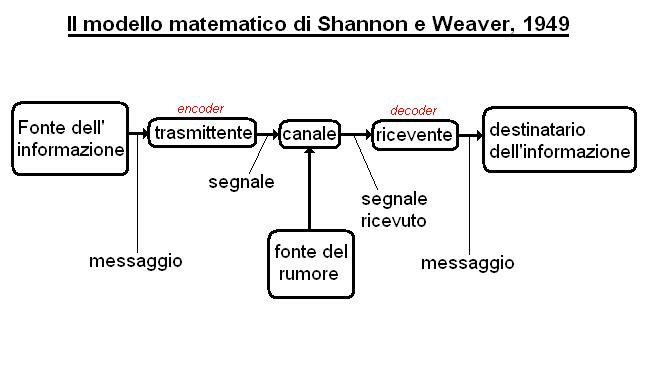
\includegraphics[width=\linewidth]{img/communication-model.jpg}
    \caption{Modello della comunicazione.}
    \label{fig:communication-model}
\end{figure}

La comunicazione è strutturata in cinque fasi:
\begin{enumerate}
    \item codifica di sorgente: il mittente rimuove la ridondanza dal messaggio.
    Di fatto, il messaggio viene compresso in maniera loss-less.
    \item codifica di canale: il mittente aggiunge ridondanza mirata al messaggio
    compresso, in modo da permettere al destinatario di rilevare e correggere
    eventuali errori presenti nel messaggio ricevuto.
    La codifica di canale è fondamentale in quanto, a seguito della
    codifica di sorgente, i bit del messaggio compresso assumono un'importanza
    maggiore rispetto a quelli del messaggio di partenza, in quanto sono
    in numero ridotto rispetto ad essi, ma trasportano la stessa quantità di
    informazione. La perdita o modifica di uno di questi bit, quindi,
    porterebbe a importanti modifiche nell'informazione trasmessa e quindi
    a una grave distorsione.
    \item trasmissione su canale, e quindi introduzione di errori nel messaggio,
    causati dal rumore.
    \item decodifica di canale: il destinatario verifica se il messaggio ricevuto
    è afflitto da errori, ed eventualmente li corregge.
    \item decodifica: il messaggio ricevuto e corretto viene decompresso,
    in modo che il destinatario ottenga il messaggio originale.
\end{enumerate}

Questi principi non sono del tutto estranei a fenomeni reali e "naturali":
il linguaggio umano, infatti, prevede che le parole più usate siano
molto spesso quelle più corte, e che il destinatario possa capire il senso
di una frase anche se alcune sue parole vadano perse, sia in una comunicazione
orale che in una comunicazione scritta.

La teoria dell'informazione può essere utilizzata anche in altri campi
diversi dalla comunicazione fisica su canale tra due entità: ad esempio,
essa permette di modellare correttamente l'evoluzione, nel corso del tempo,
di un messaggio che si trova nello stesso posto, impresso su un mezzo fisico.
Un esempio può essere un uomo primitivo che incide una pietra: esso si comporta
come il mittente, che "invia" il messaggio sulla pietra, ovvero lo incide;
nel corso del tempo, però, il messaggio inciso viene modificato da fenomeni
naturali (rumore). Il destinatario è colui che osserva le incisioni dopo
moltissimi tempo, come ad esempio un archeologo.

\chapter{Apprendimento supervisionato}
L'apprendimento supervisionato, detto anche induttivo, è quel tipo di apprendimento in cui l'algoritmo elabora un'ipotesi a partire da un dataset di istanze, a ognuna delle quali è già assegnata una label indicante il corretto risultato.

Se l'ipotesi fornisce i risultati corretti per tutte le istanze di addestramento, e quindi concorda con la funzione target, allora si dice che l'ipotesi è consistente. 
Anche se un'ipotesi si rivela essere consistente, non è detto sia la più corretta: un'ipotesi dovrebbe essere, infatti, il più semplice possibile, in modo da avere maggiori capacità predittive su istanze nuove, non presenti nel dataset di apprendimento.

È importante ricordare che il dataset di addestramento non copre tutto il dominio: in questo caso, infatti, non avrebbe senso utilizzare un algoritmo di ML, in quanto basterebbe memorizzare completamente il dominio stesso.

\section{Concept learning}
Il concept learning è un tipo di apprendimento supervisionato che, come suggerisce il nome, permette all'algoritmo di apprendere un \textit{concetto}.

Di conseguenza, l'output della fase di inferenza è un valore booleano, che specifica se l'istanza di input è un esempio del concetto (valore 1) o non lo è (valore 0).

L'ipotesi $h$ è quindi una funzione booleana $n$-aria, con $n$ numero di attributi delle istanze: 
\begin{center}
    $h: A_1 \times \ldots \times A_n \rightarrow \{ 0, 1 \}$
\end{center}
Nel concept learning, un'ipotesi è rappresentata come una congiunzione di vincoli sugli attributi: un'istanza è un esempio del concetto sse rispetta tutti i vincoli.
Un vincolo può:
\begin{itemize}
    \item obbligare un attributo ad assumere un certo valore. Viene indicato con:
    \begin{center}
        \textit{nome vincolo = valore}
    \end{center}
    \item disinteressarsi del valore assunto da un attributo. Viene indicato con:
    \begin{center}
        \textit{nome vincolo = ?}
    \end{center} 
    \item obbligare un vincolo a non assumere alcun valore. Viene indicato con:
    \begin{center}
        \textit{nome vincolo = $\emptyset$}
    \end{center}
\end{itemize}
In realtà, nella fase di addestramento non viene definita una singola ipotesi $h$, ma si genera un insieme $H$ di ipotesi differenti.
Tra queste, si considerano solo quelle consistenti con il dataset di addestramento e, tra quest'ultime, si seleziona quella più semplice, che possiede quindi una maggior capacità di previsione su istanze nuove.

\subsection{Alberi di decisione}
Gli alberi di decisione sono un esempio di algoritmo di concept learning, e possono essere applicati quando:
\begin{itemize}
    \item tutti gli attributi sono definiti su domini discreti. È possibile ridursi al caso di soli attributi booleani: un attributo su dominio discreto con $n$ possibili valori può infatti essere rappresentato usando $\lceil \log_2 n \rceil$ attributi booleani;
    \item il codominio è categorico, ovvero è anch'esso discreto;
    \item il dataset di addestramento presenta errori di contraddizione: l'algoritmo può, infatti, procedere nella sua esecuzione e terminare, anche se l'affidabilità dell'ipotesi formulata non sarà garantita.
    \item alcune istanze del dataset di addestramento presentano valori mancanti.
\end{itemize}
Un albero di decisione è un albero in cui ogni nodo interno rappresenta un attributo (detto attributo di splitting), gli archi uscenti da un nodo rappresentano i possibili valori assumibili dall'attributo su cui è definito il nodo, e una foglia rappresenta la categoria a cui appartengono le istanze che rispettano tutti i vincoli specificati nel cammino radice-foglia.

Ogni ramo radice-foglia può essere rappresentato come una WFF, in particolare come una congiunzione dei vincoli che definiscono il ramo. Si può rappresentare come WFF anche il criterio con cui stabilire a quale categoria appartiene una certa istanza: esso è, infatti, una disgiunzione di tutte le WFF rappresentanti rami dell'albero di decisione che presentano la categoria stessa come nodo foglia. Un criterio di categorizzazione è quindi rappresentato come una DNF-WFF.

Detto $n$ il numero di attributi booleani che definiscono ogni istanza (non si perde di generalità, ogni attributo discreto non booleano che presenta $v$ valori può essere rappresentato con $\lceil \log_2 v \rceil$ attributi booleani), allora il numero possibile di ipotesi (e quindi alberi di decisione) che è possibile definire è pari a $2^{2^n}$: è infatti pari al numero di possibili tabelle di verità che è possibile definire su $n$ variabili booleane.
Si continuerà però a considerare anche istanze con valori discreti non booleani.

Ogni albero di decisione presenta un altezza massima pari a $n$, ovvero il numero di attributi delle istanze.
Sia invece $A$ l'insieme degli attributi e $a_i$ l'attributo di indice $i$, allora il numero massimo di rami di un albero di decisione è pari a $\prod_{i=1}^{n} |a_i|$.

L'idea è quindi quella di trovare l'albero di decisione consistente di dimensione minore, dove con dimensione si intende la sua profondità: scegliere infatti un albero poco profondo significa scegliere un'ipotesi semplice, con quindi una maggiore capacità predittiva su istanze nuove (oltre che essere computazionalmente più efficiente).
Per farlo, a ogni istante viene scelto come attributo di splitting quello che divide l'insieme delle istanze in sottoinsiemi il più possibile uniformi. Più un insieme è uniforme, infatti, meno difficile è stabilire la categoria delle sue istanze: sarà infatti necessario controllare meno attributi per stabilire a quale categoria una certa istanza appartiene, rispetto a un insieme meno uniforme.

Gli alberi di decisione presentano quindi un \textit{bias}: prediligono infatti, tra tutti gli alberi di decisione (e quindi le ipotesi che rappresentano), quelli di altezza minore. Questo bias è però solitamente fortemente desiderato, perché permette di contenere l'overfitting e di avere efficienza computazionale.

\subsubsection{Costruzione dell'albero di decisione}
L'algoritmo di costruzione dell'albero, ad un certo istante della sua esecuzione, seleziona l'attributo che permette di partizionare l'insieme delle istanze corrente in sottoinsiemi il più possibili uniformi. Partendo dalla radice, questo ragionamento viene applicato ricorsivamente a tutti i nodi dell'albero.
L'algoritmo può quindi essere riassunto come segue:
\begin{enumerate}
    \item seleziona l'attributo migliore per l'insieme delle istanze corrente;
    \item assegna l'attributo scelto al nodo corrente;
    \item per ognuno dei possibili valori assumibili dall'attributo, crea un nodo discendente del nodo corrente;
    \item partiziona l'insieme delle clausole tra i nodi discendenti, in modo che il sottoinsieme associato a un nodo discendente definito sul valore $v_i$ dell'attributo contenga solo istanze per cui l'attributo assume valore $v_i$;
    \item per ogni nodo discendente, se esso non è completamente categorizzato, allora esegue ricorsivamente l'algoritmo sul nodo discendente.
\end{enumerate}
Serve, però, un criterio con cui selezionare l'attributo migliore. I più utilizzati sono:
\begin{itemize}
    \item attributo con il maggiore \textit{information gain}.\\
    L'information gain è un concetto presente in teorema dell'informazione, e quantifica la riduzione di entropia dell'informazione che si verifica quando si viene a conoscenza dello stato di una variabile non ancora assegnata, che nel caso degli alberi di decisione corrisponde a un attributo.
    L'entropia di un sistema è la quantità di informazione che esso contiene, e si può considerare come la sua "confusione", ovvero quanto i suoi elementi sono diversi tra loro: minimizzare l'entropia significa quindi ridurre il più possibile questa confusione.
    Sempre dalla teoria dell'informazione, maggiore l'entropia, maggiore è la quantità di bit richiesti per rappresentare il sistema che si sta considerando: di conseguenza, l'entropia dell'informazione è misurata in bit.
    
    L'information gain viene calcolato come:
    \begin{center}
        $IG(T, a) = H(T) - H(T | a)$
    \end{center}
    dove $H(T)$ è l'entropia del sistema allo stato corrente, calcolata sull'attributo $T$, $H(T | a)$ è l'entropia del sistema, calcolata su $T$, condizionata da un altro attributo $a$, ovvero quando si è a conoscenza del valore di $a$.
    L'attributo $T$, nel caso degli alberi di decisione, coincide con l'attributo "target", ovvero il risultato associato a ogni istanza.
    
    Sia $V$ l'insieme dei possibili valori assumibili dall'attributo $T$, e $v_i$ l'$i$-esimo valore assumibile da $T$. L'entropia associata a un sistema, e calcolata sull'attributo $T$, è:
    \begin{center}
        $H(T) = -\sum\limits_{i = 1}^{|V|} \left( p(v_i) \cdot \log_2 p(v_i) \right) $
    \end{center}
    Sia invece $U$ l'insieme dei possibili valori assumibili da un altro attributo $a$, e $u_i$ l'$i$-esimo valore assumibile da $a$.
    L'entropia associata a un sistema, calcolata sull'attributo $T$ ma essendo a conoscenza del valore assunto da $a$ è:
    \begin{center}
        $H(T | a) = \sum\limits_{i = 1}^{|U|} \left( p(a = u_i) \cdot H(T | a=u_i) \right) $
    \end{center}
    dove $p(a = u_i)$ è la probabilità che $a$ assuma il valore $u_i$ (in pratica il numero di istanze che presentano $u_i$ come valore di $a$), mentre $H(T | a = u_i)$ è l'entropia del sistema, calcolata su $T$, considerando le sole istanze che presentano $u_i$ come valore di $a$.
    
    L'utilizzo dell'entropia per la selezione del miglior attributo presenta due bias: predilige infatti alberi di decisione brevi, ovvero di piccola altezza, e pone più vicino alla radice gli attributi che presentano un maggior information gain, che quindi vengono considerati più rilevanti per la categorizzazione delle istanze.
    
    \item attributo con il miglior \textit{indice di Gini}.\\
    L'indice di Gini è un indicatore della disuguaglianza di una distribuzione.
    Può assumere valori compresi tra 0 e 1: 0 indica che la distribuzione è completamente omogenea, mentre 1 indica che la distribuzione è il più disuguale possibile.
    
    Sia $T$ la variabile target, ovvero il risultato, che può assumere $c$ valori differenti $t_i$. Esso viene calcolato come:
    \begin{center}
        $G = 1 - \sum\limits_{i=1}^{c} p_i^2$
    \end{center}
    dove $p_i$ è la probabilità che $T$ assuma il valore $t_i$.
    
    Sia $V$ l'insieme dei possibili valori assumibili da un attributo $a$, e $v_i$ l'$i$-esimo valore assumibile da $a$. L'indice di Gini del dominio conoscendo il valore assunto da $a$ viene calcolato come:
    \begin{center}
        $G_a = \sum\limits \left( p(a = v_i) \cdot G_{a = v_i} \right) $
    \end{center}
    Verrà quindi scelto, tra tutti gli attributi, l'attributo $s$ che minimizza l'indice di Gini complessivo dei sottoinsiemi di istanze.
    \begin{center}
        $s : s \in A \land G_s = \textnormal{min}\left\{ G_a | a \in A \right\}$
    \end{center}
\end{itemize}
L'algoritmo per la generazione di un albero di decisione è un algoritmo greedy: a ogni passo viene infatti scelto l'attributo con il maggior information gain/minor indice di Gini. Questo algoritmo greedy non porta però alla soluzione ottimale: potrebbe infatti esistere un albero di altezza minore. Tendenzialmente, però, l'albero costruito è un buon albero, e approssima bene la soluzione ottima.

Presenta inoltre il vantaggio di poter sopportare errori di contraddizione nel dataset.

\clearpage

\section{Neuroni}
Nel corso degli anni, sono stati sviluppati nuovi algoritmi di apprendimento di ispirazione biologica, in particolare ispirati al cervello.
I neuroni di ML non sono però vere e proprie modellazione di neuroni reali, ma sono semplicemente dei modelli che ne mimano il comportamento.

\subsection{Percettrone}
Un percettrone è formalmente definito come una quadrupla:
\begin{center}
    $\langle n, \Vec{c}, \Vec{w}, \theta \rangle$
\end{center}
dove:
\begin{itemize}
    \item $n$ è l'identificatore univoco del neurone;
    \item $\Vec{c}$ è il vettore di connessioni in ingresso;
    \item $\Vec{w}$ è il vettore dei pesi delle connessioni in ingresso;
    \item $\theta$ è la soglia di attivazione, ovvero il valore minimo necessario per eccitare la connessioni in uscita.
\end{itemize}

\begin{figure}[h]
    \centering
    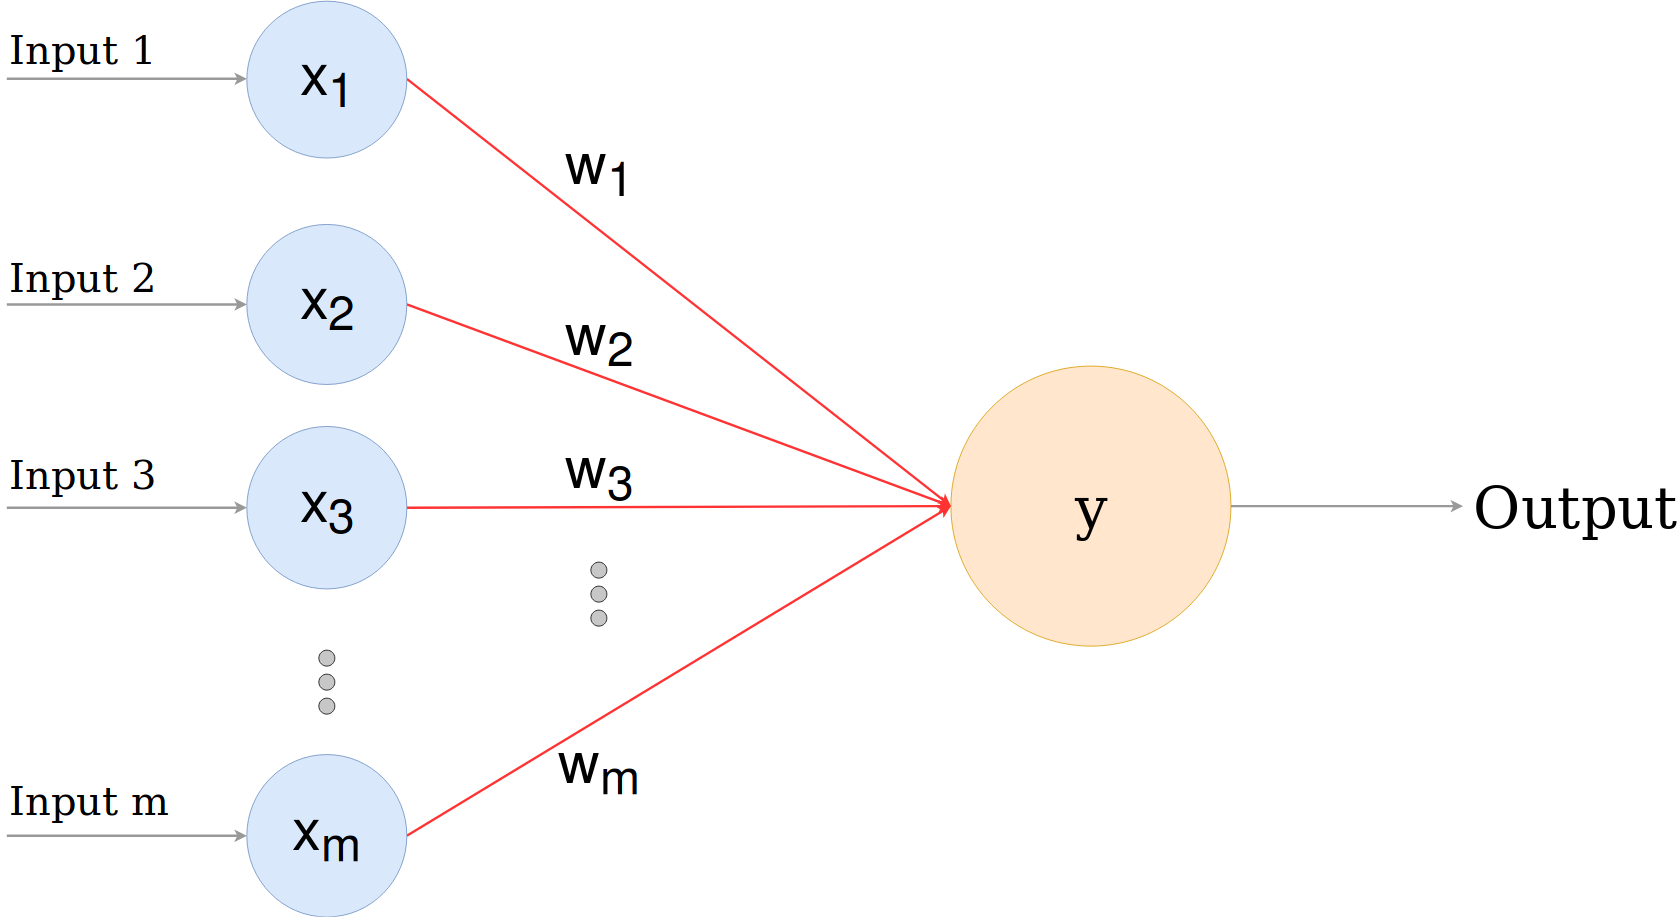
\includegraphics[width=0.7\linewidth]{images/perceptron.png}
    \caption{Struttura di un percettrone}
    \label{fig:perceptron}
\end{figure}
Un percettrone si può quindi considerare come una rete neurale unitaria e binaria, che quindi classifica l'istanza di input: se infatti la connessione in uscita è eccitata, allora il percettrone categorizza positivamente l'istanza; se invece la connessione in uscita non viene eccitata, allora l'istanza è categorizzata negativamente.
A differenza degli alberi di decisione, però, il percettrone supporta \textit{input continui}.

Il percettrone può categorizzare correttamente le istanze sse esse sono linearmente separabili in $n$ dimensioni, dove $n$ è il numero di connessioni in ingresso. Se esse sono linearmente separabili, allora esiste un iperpiano in $n-1$ dimensioni che divide correttamente lo spazio delle istanze.
Un percettrone rappresenta l'iperpiano tramite i propri  pesi di ingresso: la loro modifica nella fase di apprendimento, quindi, non fa altro che spostare l'iperpiano nello spazio delle istanze fino a quando, idealmente, si riesce a separare linearmente tutte le istanze.
\begin{figure}[h]
    \centering
    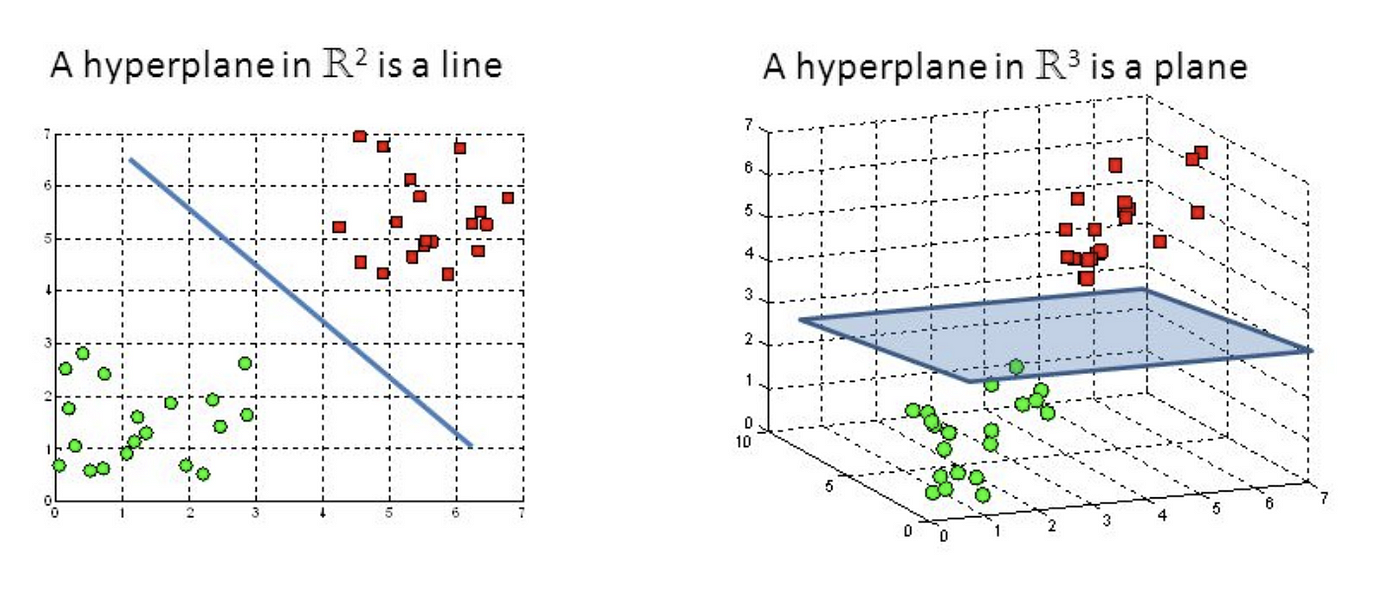
\includegraphics[width=1\linewidth]{images/hyperplane_perceptron.png}
    \caption{Iperpiani definiti da un percettrone in due differenti casi in cui le istanze sono linearmente separabili.}
    \label{fig:hyperplane_perceptron}
\end{figure}
In un percettrone, l'ipotesi coincide con l'iperpiano ed è quindi di fatto rappresentata dai pesi, che vengono modificati nel corso della fase di apprendimento.

\subsubsection{Inferenza}
La computazione del neurone all'istante di tempo $t$ avviene, una volta ricevuti gli input, effettuando la somma pesata degli input, ovvero calcolando la funzione:
\begin{center}
    $\sum\limits_{i = 1}^{n} (c_i(t) \cdot w_i(t))$
\end{center}
Sia $u$ la connessione in uscita, allora il valore assunto da $u$ sarà:
\begin{center}
    $f(\Vec{c}, \Vec{w}, \theta, t) = \begin{cases}
        1 & \sum\limits_{i = 1}^{n} (c_i(t) \cdot w_i(t)) - \theta \ge 0 \\
        0 & \textnormal{altrimenti}
    \end{cases}$
\end{center}
Di conseguenza, lo stato della connessione in uscita è determinato da una \textit{funzione a gradino}.

\subsubsection{Apprendimento}
L'apprendimento del percettrone avviene, invece, modificando i pesi associati alle connessioni di input.
Sia $w^t$ il vettore dei pesi all'istante $t$, allora $w^{t+1}$, ovvero il vettore dei pesi all'istante successivo, sarà:
\begin{center}
    $w^{t+1} = w^t + \eta \cdot (t(c^t) - h(c^t)) \cdot c^t$
\end{center}
dove $\eta$ è la costante di apprendimento, $t(c^t)$ è il valore calcolato dalla funzione target (ovvero il risultato atteso) sugli input $c^t$, e $h(c^t)$ è il valore calcolato dall'ipotesi corrente sugli input $c^t$.\\
$t(c^t) - h(c^t)$ può quindi essere considerato come l'errore di previsione. Se l'output è corretto, allora $t(c^t) - h(c^t) = 0$ e i pesi non verranno modificati.

Nel percettrone, in realtà, anche la soglia $\theta$ viene modificata nel corso dell'apprendimento: questo corrisponde, di fatto, allo spostamento dell'iperpiano definito dai pesi sulle connessioni di input.
Potendo l'algoritmo modificare solo il vettore dei pesi $w$, per modificare la soglia non si fa altro che aggiungerla come peso $w_0$ su una connessione di input $c_0$ fittizia. Aumentare il numero di connessioni in ingresso significa, però, aumentare il numero di dimensioni in cui si sta operando: sia $n$ il numero di connessioni di ingresso, l'aggiunta di $\theta$ come peso fittizio porterà l'algoritmo a lavorare in $n+1$ dimensioni.
Il valore di input $c_0$ ricevuto sulla connessione fittizia ad un certo istante di tempo $t$ è costante: solitamente, però, viene posto -1 o 1, ed in entrambi i casi l'algoritmo converge se le precedenti condizioni sono rispettate.

L'apprendimento del percettrone converge, ovvero smette di sbagliare sulle istanze di apprendimento, sse i dati sono linearmente separabili e la costante di apprendimento $\eta$ è abbastanza piccola.
Se quindi le istanze non sono linearmente separabili, l'addestramento del percettrone non termina mai.

\subsection{Reti neurali}
Le reti neurali sono un algoritmo di apprendimento di fatto implementato come un insieme di neuroni connessi tra loro.
Una rete neurale è composta da strati di neuroni, i quali possono essere divisi in tre parti:
\begin{itemize}
    \item strato di input: neuroni che ricevono l'input della rete neurale, che può essere un'istanza del dataset in fase di apprendimento o l'istanza di cui si vuole fare la previsione in fase di inferenza.
    \item strati nascosti: neuroni interni alla rete neurale, che di fatto permettono di definire una curva di separazione dello spazio delle istanze anzichè un semplice iperpiano.
    \item strato di output: neuroni che forniscono l'output della rete neurale.
\end{itemize}
\begin{figure}[h]
    \centering
    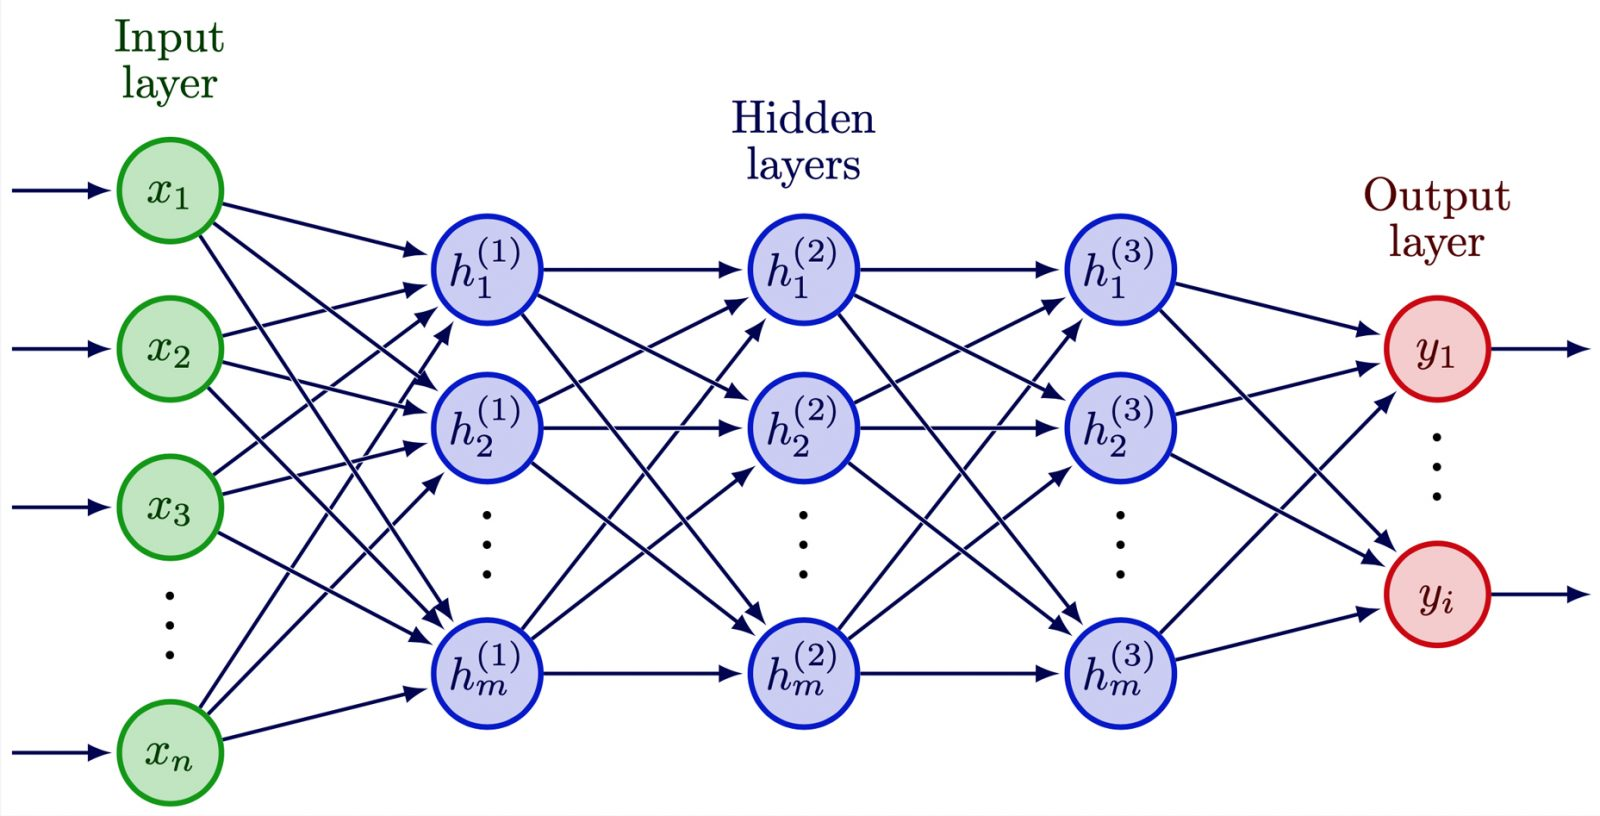
\includegraphics[width=0.75\linewidth]{images/neural_network.jpg}
    \caption{Struttura di una rete neurale}
    \label{fig:neural_network}
\end{figure}
Se tutti i neuroni sono percettroni, allora si parla di multilayer perceptron.

Nelle reti neurali, ogni neurone mantiene un proprio vettore dei pesi sulle proprie connessioni di input.
Il vettore pesi di un singolo neurone non viene però aggiornato immediatamente a seguito dell'elaborazione, da parte del neurone, del suo output, ma la rete neurale "ragiona" nella sua totalità: si aspetta quindi che l'intera rete neurale fornisca l'output (tramite i neuroni dello strato di output), per poi calcolare un errore sulla previsione della rete, e infine correggere i pesi di tutti i neuroni della rete retroattivamente attraverso un algoritmo di backpropagation.

Si consideri ora una rete di questo tipo, con un singolo neurone di output che ha $n$ connessioni di input, a loro volta connessioni di output di $n$ neuroni.
IMMAGINE
L'errore del neurone, ovvero la differenza tra output atteso da quel nodo e output effettivamente fornito, viene calcolato con una loss function $L(\Vec{w})$. Esistono diverse loss function, una delle più usate è quella basata sullo scarto quadratico:
\begin{center}
    $L(\Vec{w}) = \frac{1}{2} \cdot \left( y(\Vec{w})- t(\Vec{w}) \right)^2$
\end{center}
dove $y(\Vec{w})$ è la previsione effettuata dall'ipotesi corrente e $t(\Vec{w})$ è la previsione corretta, ovvero il valore calcolato dalla funzione target.
Essendo però $y(\Vec{w})$ e $t(\Vec{w})$ due funzioni dipendenti dal vettore dei pesi, allora anche la loss function dipenderà dai pesi $\Vec{w}$ delle connessioni in ingresso al nodo.

Una volta calcolata la loss function, i pesi delle connessioni in ingresso al neurone vengono aggiornati nel seguente modo:
\begin{center}
    $\Vec{w}_{fin} = \Vec{w}_{iniz} - \eta \cdot \nabla L(\Vec{w}_{iniz})$
\end{center}
dove $\eta$ è il tasso di apprendimento, $\nabla L(\Vec{w}_{iniz})$ è il gradiente della loss function calcolato nel punto $\Vec{w}_{iniz}$.

La loss function viene calcolata per ogni neurone, e il relativo aggiornamento dei pesi può essere effettuato solo sulle connessioni in ingresso al neurone considerato.
Se i neuroni precedenti presentano a loro volta dei neuroni precedenti, come nel caso di reti neurali con più strati, allora è necessario applicare ricorsivamente questo ragionamento per ognuno dei nodi precedenti e così via, fino ai neuroni dello strato di input compresi.
Quando si fa questa cosa sui nodi precedenti, deve essere definito un nuovo concetto di errore di previsione. In questo caso, infatti, la previsione effettuata dal nodo è il valore fornito in output al neurone da cui si è provenuti per il vecchio peso associato a quella connessione, mentre la previsione corretta è sempre lo stesso output ma moltiplicato per il peso corretto quando ci si trovava ancora nel neurone da cui si è provenuti.

Utilizzando il gradiente della funzione errore, e volendo minimizzare la loss function proprio analizzando il gradiente (che definisce la miglior direzione di discesa, mentre lo step è dettato dal tasso di apprendimento), allora l'algoritmo di apprendimento adottato dalle reti neurali viene detto anche discesa del gradiente.

Dovendo calcolare il gradiente della loss function, ed essendo la loss function definita come $h(\Vec{c}) - t(\Vec{c})$, allora sia $h(\Vec{c})$ che $t(\Vec{c})$ devono essere derivabili. Si suppone la funzione target $t$ sia derivabile. $h(\Vec{c})$ deve essere derivabile: non è quindi possibile utilizzare come funzione di attivazione di un neurone una funzione a step (lo step non è derivabile) e bisogna utilizzare un'altra funzione, come la funzione sigmoide $f(x) = \frac{1}{1+e^{-x}}, x = \sum_i w_i \cdot s_i$.

A inizio apprendimento, tutti i pesi della rete neurale vengono inizializzati casualmente.

La correzione dei pesi può avvenire in tre modi:
\begin{itemize}
    \item modalità batch: vengono elaborate tutte le istanza del dataset di apprendimento, per poi calcolare l'errore di previsione sull'intero dataset.
    \item modalità incrementale: viene elaborato solo un sottoinsieme delle istanze del dataset di apprendimento, per poi calcolare l'errore solo sul sottoinsieme di istanze elaborato.
    \item modalità stocastica: a seguito dell'elaborazione di ogni singola istanza, viene calcolato l'errore solo su quella istanza.
\end{itemize}
\begin{figure}
    \centering
    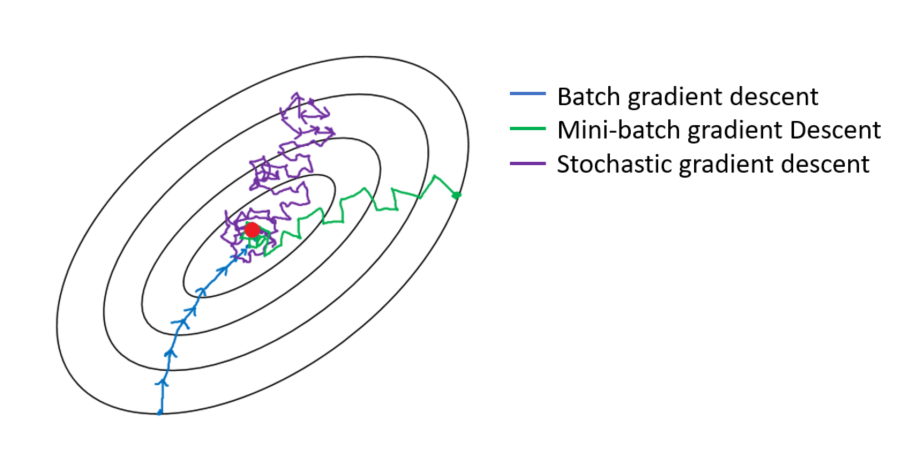
\includegraphics[width=0.75\linewidth]{images/gradient_descent.png}
    \caption{Caption}
    \label{fig:gradient_descent}
\end{figure}
La modalità batch è quella che permette di correggere al meglio i pesi dei neuroni. La modalità incrementale non è altro che un approssimazione della modalità batch: più il sottoinsieme di istanze considerato è grande, migliore sarà la correzione dei pesi della rete neurale. Essendo però un approssimazione, la modifica dei pesi muove in maniera peggiore il punto identificato dai pesi nello spazio, e non è quindi il miglior spostamento verso il minimo.
La modalità stocastica è la peggiore, e viene solitamente evitata.

Una sola correzione non basta per trovare l'ipotesi desiderata: effettuare una volta una correzione dei pesi di tutta la rete, anche se ciò viene fatto in modalità batch, non assicura che tutte le istanze di validazione siano poi effettivamente inferenziate correttamente.
Infatti, una correzione rappresenta semplicemente uno step sulla loss function, ma potrebbero essere necessari più step per raggiungere effettivamente il minimo.
Possono essere quindi necessarie più correzioni, ognuna delle quali prende il nome di epoca.
Il numero di epoche è dettato dalla dimensione del tasso di apprendimento.

Una rete neurale utilizza anche altre tecniche per permettere un migliore apprendimento.
Il primo problema che si deve cercare di risolvere è il valore assunto dal tasso di apprendimento: se infatti risulta troppo grande, allora lo step di discesa risulta ampio, con quindi un apprendimento più rapido ma meno preciso.
Se invece il tasso di apprendimento è piccolo, allora l'apprendimento sarà preciso, ma sarà molto più lento nel assestarsi su un minimo.
Un tasso di apprendimento piccolo può portare inoltre all'assestamento su minimi locali: uno step ampio permetterebbe infatti di evitarli, mentre quello piccolo no.
La tecnica che si adotta è quindi di mantenere ampio il tasso di apprendimento all'inizio dell'apprendimento, e man mano diminuirlo al procedere dell'apprendimento.

L'algoritmo di discesa del gradiente (che è un algoritmo di apprendimento) converge, ovvero termina di imparare, solo se il tasso di apprendimento è basso: un ampio step potrebbe infatti portare nelle vicinanze del minimo locale, ma poi continuare a "saltare" intorno ad esso senza mai riuscire effettivamente a fermarsi sul minimo.

Dato un certo dataset e qualsiasi sia l'algoritmo di apprendimento usato, solitamente il dataset viene diviso in tre sottoinsiemi: istanze di apprendimento, istanze di validazione e istanze di test.
Le istanze di test, usate alla fine dell'apprendimento, permettono di stabilire se il modello appreso prevede bene istanze nuove mai usate nell'addestramento, ovvero quelle rappresentate dalle istanze di test.
Nel caso in cui si consideri bello il modello, allora tutto a posto. Nel caso in cui invece si rilevi, eseguendo il modello sulle istanze di test, che il modello non va bene, allora viene scartato e si riparte.
Nel caso delle reti neurali, ricominciare significa generare nuovi pesi casuali diversi dai precedenti e ripetere l'addestramento.



Le reti neurali sono abbastanza lente nell'addestramento (comunque più veloci del deep learning) ma sono abbastanza efficienti e veloci nella fase di inferenza. 

\section{Support Vector Machine}
Il Support Vector Machine (SVM) è un algoritmo di classificazione che permette di separare le istanze usando funzioni non lineare. Come si vedrà, in realtà SVM non definisce funzioni non lineari, ma definisce funzioni lineari in dimensioni superiori che si traducono in funzioni non lineari in dimensioni inferiori. 

\subsubsection{Perchè usare le SVM, e alcune loro limitazioni}
Le reti neurali a singolo strato permettono di definire funzioni di separazione lineari (iperpiani) efficientemente. Se però le istanze non sono linearmente separabili, allora possono essere utilizzate le reti neurali multistrato, che permettono di definire funzioni non lineare in maniera, però, poco efficiente.\\
Le SVM individuano funzioni di separazione non lineare più efficientemente delle reti neurali. Risolvono inoltre un altro problema, che riguarda l'ottimizzazione: le reti neurali, infatti, apprendono cercando di risolvere un problema di ottimizzazione non convessa non vincolata, il quale presenta molti punti di minimo locali. Le SVM, invece, apprendono risolvendo un problema di ottimizzazione quadratico convesso, che presenta un solo minimo globale: non si presenta quindi il rischio di assestarsi su minimi locali durante l'apprendimento.

Le SVM presentano comunque delle limitazioni. Innanzitutto, richiedono che tutte le istanze di addestramento siano classificate, cosa non sempre vera in un dataset.
Inoltre, le SVM possono essere utilizzate solo in problemi di classificazione binari. Se si desidera poter classificare un'istanza in più di due classi, allora il problema deve essere ridotto a problemi di classificazione binari multipli \footnote{Vedere: multi-class SVM.}.
Infine, il modello individuato da una SVM offre una buona generalizzazione solo se il dataset di addestramento è stato standardizzato \footnote{Vedere: min-max, Z-score, sottrazione della media e divisione per la varianza.}

\subsubsection{Iperpiani separatori e margine}
Quando si vogliono dividere le istanze usando un iperpiano \footnote{Un iperpiano è una funzione lineare.}, è possibile che più iperpiani diversi le possano dividere correttamente.
Non tutti gli iperpiani hanno però la stessa capacità di generalizzare, e ciò si ripercuoterà sulla fase di inferenza di nuove istanze.
\begin{figure}[h]
    \centering
    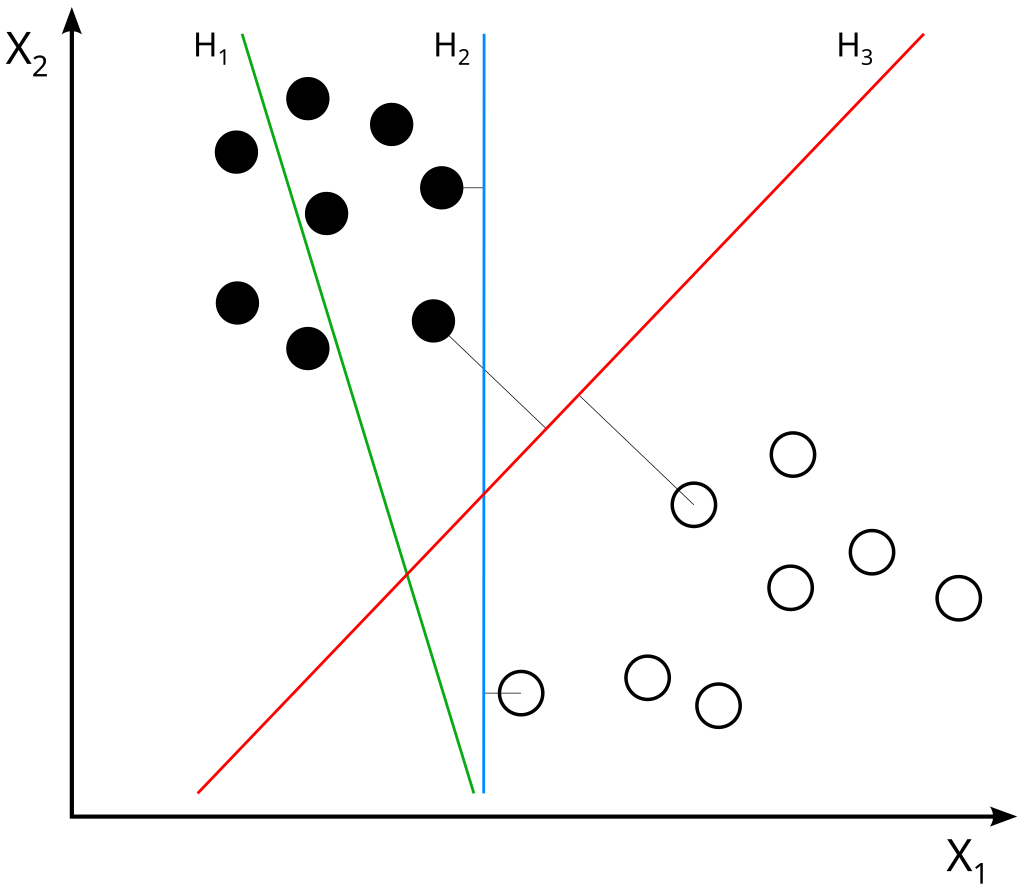
\includegraphics[width=0.5\linewidth]{images/hyperplanes.png}
    \caption{$H_1$ non divide correttamente le istanze. $H_2$ divide correttamente le istanze, ma ha un piccolo margine. $H_3$ divide correttamente le istanze ed ha un margine ampio.}
    \label{fig:svm_margin}
\end{figure}
\begin{defn}
    Il \textbf{margine} (geometrico) $\gamma$ di un iperpiano $w$ che divide le istanze è METTERE DEFINIZIONE DI MARGINE. 

    Il margine positivo $\gamma^+$ dell'iperpiano $w$ indica la minima distanza perpendicolare tra un'istanza classificata positivamente e l'iperpiano $w$, mentre il margine negativo $\gamma^-$ indica la minima distanza perpendicolare tra un'istanza classificata negativamente e l'iperpiano $w$.\\
    Il margine "generale" $\gamma$ dell'iperpiano $w$ equivale semplicemente a $\gamma = \gamma^+ + \gamma^-$.
\end{defn}
Viene dimostrato \footnote{Vedere: Teoria statistica dell'apprendimento, dimensione di Vapnik-Cervonenkis} che l'iperpiano che permette di avere la generalizzazione massima, ovvero quello che permette al modello di massimizzare il numero di previsioni corrette su nuove istanze nella fase di inferenza, è quello che massimizza il margine.

\subsubsection{Trovare il miglior iperpiano}
Ogni iperpiano può essere univocamente identificato da un vettore normale \footnote{Con vettore normale si intende un qualsiasi vettore perpendicolare all'iperpiano, non necessariamente di lunghezza unitaria. Se il vettore ha anche lunghezza unitaria, allora si dice che è normalizzato.} e uno scalare $b$.
$\Vec{w}$ definisce l'orientamento dell'iperpiano, mentre $b$ permette di calcolare l'offset dell'iperpiano rispetto all'origine lungo il vettore normale come $\frac{b}{\norm{\Vec{w}}}$.\\
L'equazione che descrive l'iperpiano è quindi:
\begin{equation*}
    \Vec{w}^T \Vec{x_i} + b = 0
\end{equation*}

Per ogni iperpiano $w$, è possibile definire due ulteriori iperpiani a lui paralleli. Questi due iperpiani sono descritti dalle equazioni:
\[
    w^+: \Vec{w}^T \cdot \Vec{x_i} + b = 1 \quad \quad w^-: \Vec{w}^T \cdot \Vec{x_i} + b = -1
\]
La distanza geometrica tra questi due iperpiani \footnote{Essendo paralleli, questa distanza è stata calcolata con la formula per la distanza tra punto e piano.} è pari a $\frac{2}{\norm{\Vec{w}}}$.\\
Ma la distanza tra questi due iperpiani è proprio il margine, che vogliamo massimizzare.
Di conseguenza vogliamo risolvere il seguente problema di ottimizzazione \footnote{Si può notare che all'aumentare di $\norm{\Vec{w}}$ il margine diminuisce, e quindi gli iperpiani paralelli si avvicinano all'iperpiano separatore. Viceversa, al diminuire di $\norm{\Vec{w}}$ gli iperpiani paralleli si allontanano.}:
\begin{maxi*}|s|[1]
    {\Vec{w}, b}{\frac{2}{\norm{\Vec{w}}}}
    {}{}
\end{maxi*}

L'iperpiano fino ad ora definito e i relativi iperpiani paralleli, però, non tengono conto della corretta classificazione delle istanze. L'individuazione dell'iperpiano ne deve tenere conto per un corretto apprendimento. Di conseguenza, gli iperpiani desiderati devono essere considerati solo tra quelli che classificano correttamente le istanze.\\
Devono essere quindi aggiunti due vincoli:
\[
    \bra{\Vec{w}^T \cdot \Vec{x_i} + b} \ge 1 \tn{ se } y_i = 1 \quad \quad \bra{\Vec{w}^T \cdot \Vec{x_i} + b} \le -1 \tn{ se } y_i = -1
\]
Il primo richiede che le istanze positive ($y_i = 1$) siano classificate correttamente, ovvero che risiedano al di sopra di $w^+$, mentre il secondo richiede che le istanze negative ($y_i = -1$) siano classificate correttamente, ovvero che risiedano al di sotto di $w^-$. \\
Questi due vincoli, inoltre, impongono che le istanze non si trovino nella regione di spazio compresa tra i due piani.\\
Ma i due vincoli possono essere uniti ed essere espressi come:
\begin{equation*}
    y_i \cdot \bra{\Vec{w}^T \cdot \Vec{x_i} + b} \ge 1
\end{equation*}

Il problema di ottimizzazione completo per l'individuazione dell'iperpiano che massimizza il margine è quindi:
\begin{maxi*}|s|
    {\Vec{w}, b}{\frac{2}{\norm{\Vec{w}}}}
    {}{}
    \addConstraint{y_i \cdot \bra{\Vec{w}^T \cdot \Vec{x_i} + b} \ge 1}
\end{maxi*}
Questo problema di massimizzazione può però essere difficile da risolvere. Si può quindi risolvere \footnote{Essendo un problema di programmazione non lineare vincolata, deve essere risolto usando i moltiplicatori di Lagrange.} il suo problema duale, conservando lo stesso vincolo per la corretta classificazione delle istanze:
\begin{mini*}|s|
    {\Vec{w}, b}{\frac{1}{2}\norm{\Vec{w}}^2}
    {}{}
    \addConstraint{y_i \cdot \bra{\Vec{w}^T \cdot \Vec{x_i} + b} \ge 1}
\end{mini*}
I $\Vec{w}$ e $b$ che risolvono questo problema determineranno l'iperpiano che massimizza il margine.

Si può notare, però, che per ogni iperpiano che divide correttamente le istanze, almeno due istanze giacciono sulla frontiera del margine: su un lato del margine risiederà almeno un'istanza classificata negativamente, mentre sull'altro almeno una che verrà classificata positivamente.
Ma le istanze che giacciono sulla frontiera identificano univocamente l'iperpiano, e di conseguenza esso può essere rappresentato anche come una somma pesata di tutte le istanze, dove i pesi saranno non nulli solo per le istanze che giacciono sulla frontiera.
\[
    \Vec{w} = \sum\limits_{i \in Q} \alpha_i \Vec{x_i}
\]
Le istanze (che non sono altre che vettori) che risiedono sulla frontiera prendono il nome di \textbf{support vectors}.\\
Essendo l'ipotesi sull'istanza $\Vec{x}$ calcolata dalla SVM come:
\[
    h(\Vec{x}) = \tn{sign}(\Vec{w}^T \cdot \Vec{x} + b)
\]
e potendo scrivere $\Vec{w}$ come $\Vec{w} = \sum\limits_{i \in Q} \alpha_i \Vec{x_i}$, allora la funzione di decisione di una SVM può essere calcolata come:
\[
    h(\Vec{x}) = \tn{sign}\bra{\sum\limits_{i \in Q} (\alpha_i \cdot \Vec{x_i} \cdot \Vec{x}) + b}
\]

\subsubsection{Soft margin}
La ricerca dell'iperpiano che massimizza il margine prevede che l'iperpiano classifichi correttamente tutte le istanze. In alcuni casi, però, il dataset potrebbe non essere linearmente separabile.\\
Viene quindi introdotto il concetto di soft margin, un particolare tipo di margine che tollera la non corretta classificazione di un numero limitato di istanze.

Per poterlo spiegare è però prima necessario introdurre la funzione di \textbf{hinge loss}: questa funzione restituisce $0$ se l'istanza $x_i$ viene classificata correttamente \footnote{L'istanza è classificata correttamente se $\Vec{w}^T \cdot \Vec{x_i} + b = y_i$. Essendo però $1$ e $-1$ gli unici valori possibili per una previsione, l'istanza è classificata correttamente anche se $y_i \cdot (\Vec{w}^T \cdot \Vec{x_i} + b) = 1$}, altrimenti restituisce un valore proporzionale alla sua distanza dal margine.
\[
    \max \bra{0, \; 1 - y_i \cdot (\Vec{w}^T \cdot \Vec{x_i} + b)}
\]
Dato un iperpiano, il valore della funzione di hinge loss calcolato per l'istanza $x_i$ viene indicato con $\zeta_i$ e prende il nome di \textbf{slack}. Lo slack associato a un'istanza deve essere sicuramente positivo.

Modificando l'iperpiano, gli slack delle varie istanze cambiano. Non conoscendo quindi il loro valore, essi si comportano come variabili di cui si deve stabilire il valore. Volendo inoltre una classificazione il più possibile corretta, si vuole minimizzare la somma di tutti gli slack \footnote{Uno slack può infatti essere visto come un errore di previsione sull'istanza.}.
Di conseguenza, il nuovo problema di ottimizzazione che si deve risolvere è:
\begin{mini*}|s|
    {\Vec{w}, b, \zeta}{\frac{1}{2}\norm{\Vec{w}}^2 + C \cdot \sum\limits_{i=1}^n \zeta_i}
    {}{}
    \addConstraint{y_i \cdot \bra{\Vec{w}^T \cdot \Vec{x_i} + b} \ge 1 - \zeta_i \quad \forall 1 \le i \le n}
    \addConstraint{\zeta_i \ge 0 \quad \forall 1 \le i \le n}{}
\end{mini*}
dove $C$ è un trade-off tra la dimensione del margine e il numero di istanze non classificate correttamente. Per alti valori di $C$, se le istanze sono linearmente separabili, l'algoritmo apprende in maniera identica a come avviene nel caso del margine rigido. Se invece le istanze non sono linearmente separabili, l'algoritmo riesce comunque a trovare una separazione lineare che minimizza l'errore. 

\subsubsection{Kernel trick (sistemare indici nei problemi di ottimizzazione)}
L'algoritmo SVM "puro" non può trovare una funzione che separa correttamente le istanze se esse non sono linearmente separabili. Il soft margin permette comunque di apprendere, ma compie errori di previsione su un un numero limitato di istanze.

Se però si vuole una classificazione corretta di tutte le istanze, e le istanze non sono linearmente separabili, allora è possibile utilizzare una tecnica chiamata \textbf{kernel trick} \footnote{Vedere: Aizerman et al.}.\\
Istanze che non sono linearmente separabili in $n$ dimensioni, infatti, saranno sicuramente separabili per un qualche $m > n$, ovvero in dimensioni superiori \footnote{In generale, $n$ istanze sono quasi sempre separabili in spazi con un numero di dimensioni maggiore o uguale a $n-1$.}.

Per spostarsi in dimensioni superiori, deve essere stabilita una funzione $\Phi$ che definisca come calcolare i valori associati alle $m$ dimensioni a partire dalle $n$ dimensioni delle istanze.
Una volta trovata la funzione $\Phi$ che permette di mappare le istanze in dimensioni superiori e di renderle linearmente separabili, il problema di ottimizzazione che si vuole risolvere diventa:
\begin{mini*}|s|
    {\Vec{w}, b, \zeta}{\frac{1}{2}\norm{\Vec{w}}^2 + C \cdot \sum\limits_{i=1}^n \zeta_i}
    {}{}
    \addConstraint{y_j \cdot \bra{\sum\limits_{i \in Q} \bra{\alpha_i \cdot \Phi(\Vec{x_i}) \cdot \Phi(\Vec{x_j})} + b} \ge 1 - \zeta_j \quad \forall 1 \le j \le n}
    \addConstraint{\zeta_i \ge 0 \quad \forall 1 \le i \le n}{}
\end{mini*}
La classificazione di un'istanza può essere decisa con la funzione:
\[
    h(\Vec{x}) = \tn{sign} \bra{\sum\limits_{i \in Q} \bra{\alpha_i \cdot \Phi(\Vec{x_i}) \cdot \Phi(\Vec{x})} + b}
\]
La funzione $\Phi$ trovata è molto spesso computazionalmente onerosa. Calcolarla quindi sull'istanza e su ogni support vector porterebbe a una fase di addestramento e una fase di inferenza lente.\\
Si può notare però che, in molti casi, il prodotto $\Phi(\Vec{x_i}) \cdot \Phi(\Vec{x})$ in $m$ dimensioni può essere espresso come una funzione $K(\Vec{x_i}, \Vec{x})$, calcolata quindi in uno spazio a $n$ dimensioni.
La funzione $K(x, y)$ prende il nome di \textbf{kernel}.

Il problema di ottimizzazione può quindi essere riscritto come:
\begin{mini*}|s|
    {\Vec{w}, b, \zeta}{\frac{1}{2}\norm{\Vec{w}}^2 + C \cdot \sum\limits_{i=1}^n \zeta_i}
    {}{}
    \addConstraint{y_j \cdot \bra{\sum\limits_{i \in Q} \bra{\alpha_i \cdot K(\Vec{x_i},  \Vec{x_j})} + b} \ge 1 - \zeta_j \quad \forall 1 \le j \le n}
    \addConstraint{\zeta_i \ge 0 \quad \forall 1 \le i \le n}{}
\end{mini*}

La funzione di decisione per un'istanza $x_i$ può essere calcolata come:
\[
    h(\Vec{x}) = \tn{sign} \bra{\sum\limits_{i \in Q} \bra{\alpha_i \cdot K(\Vec{x_i}, \Vec{x})} + b}
\]
Non dovendo più calcolare la funzione $\Phi$, l'addestramento e l'inferenza della SVM rimangono computazionalmente efficienti.

Bisogna però evidenziare che all'aumentare della dimensionalità dello spazio delle istanze, l'\textbf{errore di generalizzazione} aumenta, ovvero diminuisce la capacità di generalizzazione della SVM su nuove istanze. Nonostante ciò, una SVM addestrata su un numero adeguato di istanze mantiene una buona capacità di generalizzazione anche se utilizza kernel non lineari per l'apprendimento.

I kernel più utilizzati sono:
\begin{itemize}
    \item lineare: $K(\Vec{x}, \Vec{y}) = \Vec{x} \cdot \Vec{y}$
    \item polinomiale: $K(\Vec{x}, \Vec{y}) = (\Vec{x} \cdot \Vec{y} + r)^d$
    \item RBF gaussiano: $K(\Vec{x}, \Vec{y}) = e^{-\gamma \cdot \norm{\Vec{x} - \Vec{y}}^2}$ dove solitamente $\gamma = \frac{1}{2\sigma^2}$
    \item tangente iperbolica: $K(\Vec{x}, \Vec{y}) = \tanh (\kappa \cdot (\Vec{x} \cdot \Vec{y}) - c), \quad \kappa > 0 \land c < 0$
\end{itemize}

\subsubsection{Stabilire i parametri}
I parametri che devono essere stabiliti prima di eseguire l'algoritmo SVM su un dataset sono il trade-off $C$, il tipo di kernel $K(x, y)$ che si vuole usare ed eventualmente parametri interni al kernel.

Il kernel più utilizzato è quello gaussiano, che richiede al suo interno un ulteriore parametro $\gamma$. In questo caso, quindi, bisogna individuare solo la migliore combinazione di $C$ e $\gamma$.\\
Per farlo, si procede con una grid search di $C$ e $\gamma$: si scelgono quindi un sottoinsieme finito \footnote{Dovendo scegliere un sottoinsieme finito di possibili valori, eventuali parametri continui devono essere discretizzati.} di valori per $C$ e un sottoinsieme finito di valori per $\gamma$, e si procede con la valutazione di tutte le possibili combinazioni.
La SVM viene addestrata più volte, ogni volta usando una diversa combinazione definita con la grid search.
Una volta terminato l'addestramento per una certa combinazione, l'algoritmo ne effettua la cross validation sul sottoinsieme di istanze dedicate alla validation.
Al termine di tutti gli addestramenti sulle possibili combinazioni di parametri, l'algoritmo considera solo quello la cui combinazione di $C$ e $\gamma$ massimizza l'accuratezza di cross validation \footnote{L'accuratezza di cross validation altro non è che il numero di istanze di validazione su cui il modello trovato effettua una previsione corretta.}.

\section{Bayesian Learning}
\subsection{Introduzione}
Un algoritmo di machine learning si pone come obiettivo quello di trovare la migliore ipotesi $h \in H$ dato un dataset $D$.
Nell'apprendimento bayesiano, però, la migliore ipotesi si considera come quella più probabile tra tutte le ipotesi e, di conseguenza, sulle possibili ipotesi è definita una distribuzione di probabilità.
Questa distribuzione di probabilità sulle ipotesi viene modificata a ogni nuova istanza di addestramento incontrata, fino ad aver analizzato tutte le istanze del dataset. La distribuzione di probabilità sulle ipotesi ottenuta dopo aver analizzato l'intero dataset sarà quella che verrà usata per fare previsioni su nuove istanze.

L'aggiornamento della distribuzione viene effettuato grazie al teorema di Bayes.\\
Siano $P(h_i)$ la probabilità che l'ipotesi $h_i$ sia corretta, $P(D)$ la probabilità che il dataset sia vero e $P(D | h_i)$ la probabilità che il dataset sia vero se vale l'ipotesi $h_i$.\\
La probabilita $P(h_i | D)$ che $h_i$ sia l'ipotesi corretta dato il dataset $D$ è:
\[
    P(h_i | D) = \frac{P(D | h_i) \cdot P(h_i)}{P(D)}
\]
Si può osservare che $P(D)$ rimane costante per ipotesi differenti, e si può quindi non considerarlo quando si mettono a confronto ipotesi differenti.

Nel caso precedente si è considerato l'intero dataset $D$. Nella pratica, però, le istanze di addestramento vengono analizzate singolarmente.
Di conseguenza, il teorema viene di Bayes viene usato esattamente $|D|$ volte per aggiornare le probabilità sulle ipotesi, una per ogni istanza del dataset $D$.\\
Sia $d_j$ la $j$-esima istanza del dataset, $P(d_j)$ la probabilità che l'istanza $d_j$ sia correttamente classificata nell'universo e supponendo che siano state già analizzate le prime $i-1$ istanze del dataset (e che quindi si conoscano le probabilità $P(d_j | h_i)$ e $P(h_i)$).\\
La nuova probabilità $P(h_i | d_j)$ viene calcolata come:
\[
    P(h_i | d_j) = \frac{P(d_j | h_i) \cdot P(h_i)}{P(d_j)}
\]
Alla prima applicazione del teorema di Bayes, ovvero all'analisi della prima istanza del dataset, non si ha alcuna conoscenza sul dominio, proprio perchè il dataset non è stato ancora analizzato. Non è quindi stata ancora definita una distribuzione di probabilità sulle ipotesi.\\
Per questo motivo, le probabilità $P(h_i)$ e $P(d_j | h_i)$ vengono definite arbitrariamente. Per farlo, però, è necessario prima fare alcune assunzioni:
\begin{itemize}
    \item il dataset $D$ di addestramento non ha rumore, ovvero tutte le istanze sono classificate correttamente.
    \item la funzione target $t$ risiede nello spazio delle ipotesi $H$.
    \item non si alcuna ragione di credere che un'ipotesi sia più probabile di un'altra dato il dataset corrente.
\end{itemize}
Se queste assunzioni sono considerate, allora: 
\begin{align*}
    &P(h_i) = \frac{1}{|H|} \quad |H| \tn{ cardinalità dello spazio delle ipotesi}\\
    &P(D | h_i) = \begin{cases}
        1 & h_i(d) = t(d) \quad \forall d \in D, \tn{ ovvero $h_i$ è consistente con $D$}\\
        0 & \tn{altrimenti}
    \end{cases}\\
    &P(D) = \frac{|VS_{H,D}|}{|H|} \quad VS_{H,D} \tn{ insieme delle ipotesi consistenti con D}
\end{align*}
Calcolare la probabilità $P(h_i | D)$ è quindi molto semplice:
\begin{align*}
    P(h_i | D) = \begin{cases}
        \frac{1}{|VS_{H,D}|} & \tn{ se $h_i$ è consistente con $D$}\\
        0 & \tn{altrimenti}
    \end{cases}
\end{align*}

\subsection{Optimal Bayes Classifier}

\subsection{Naive Bayes Classifier}
Come visto nella sezione precedente, la classificazione tramite Optimal Bayes Classifier richiede alto sforzo computazionale.
Per questo motivo può essere introdotto un altro classificatore Bayesiano, chiamato Naive Bayes Classifier, che permette di trovare più facilmente la classe a cui appartiene una nuova istanza, supponendo che alcune ipotesi siano vere.

Come già visto, la classificazione di una nuova istanza $A = \langle a_1, \ldots, a_m \rangle$ può essere effettuata prendendo il valore $v_j \in V$, $V$ insieme delle classi, di massima probabilità data l'istanza.
\[
    h(\Vec{a}) = \argmax_{v_j \in V} P(v_j | \Vec{a})
\]
Per il teorema di Bayes:
\[
    h(\Vec{a}) = \argmax\limits_{v_j \in V} \frac{P(\Vec{a} | v_j) \cdot P(v_j)}{P(\Vec{a})}
\]
Ma $P(\Vec{a})$ è costante per qualsiasi $\Vec{a}$ si consideri \footnote{$P(\Vec{a}) = \frac{1}{|I|}$, con $I$ spazio delle istanze.}, e quindi si può semplificare:
\[
    h(\Vec{a}) = \argmax\limits_{v_j \in V} P(\Vec{a} | v_j) \cdot P(v_j)
\]
Stimare $P(v_j)$ è molto semplice: corrisponde infatti alla frequenza relativa di $v_j$ all'interno del dataset \footnote{In pratica, è il rapporto tra numero di istanze del dataset $D$ classificate con la classe $v_j$ e $|D|$ numero totale di istanze nel dataset.}.\\
Stimare correttamente $P(\Vec{a} | v_j)$ risulta invece più complicato, a meno che non si abbia un dataset di grandissime dimensioni.

Entra quindi in gioco un assunzione sui legami tra le feature delle istanze. L'algoritmo Naive Bayes assume che le feature siano indipendenti tra loro, e quindi:
\[
    P(\Vec{a} | v_j) = \prod\limits_{i=1}^m P(a_i | v_j) 
\]
$P(a_i | v_j)$ è molto facile da stimare: è infatti la frequenza relativa del valore $a_i$ per l'$i$-esima feature tra le sole istanze del dataset classificate con $v_j$.

Di conseguenza:
\[
    h(\Vec{a}) = \argmax\limits_{v_j \in V} \prod\limits_{i=1}^m P(a_i | v_j)  \cdot P(v_j)
\]

\subsubsection{Svantaggi del Naive Bayes Classifier}
Naive Bayes presenta alcuni svantaggi:
\begin{itemize}
    \item molto spesso gli attributi non sono indipendenti, e l'utilizzo di Naive Bayes impone quindi una indipendenza artificiosa;
    \item se l'$i$-esimo attributo non assume mai un valore nel dataset, allora $P(a_i | v_j)$ per qualsiasi valore $a_i$. Di conseguenza, tutte le classi avranno valore $0$ nella classificazione, e non si potrà quindi classificare l'istanza.\\
    Questo problema si risolve con lo smoothing, ovvero aggiungendo pochissime istanze fittizie che presentano i valori mancanti.
\end{itemize}

\subsubsection{Complessità di Naive Bayes}
Richiede di memorizzare solo $k \cdot d$ parametri, con $k$ numero di label e $d$ numero di attributi.

\subsection{Gaussian Naive Bayes Classifier}
Il Gaussian Naive Bayes Classifier è una variante di Naive Bayes che permette di trattare attributi continui.
L'utilizzo di Naive Bayes Classifier "classico" applicato su attributi continui trova infatti difficoltà a definire la probabilità $P(a_i | v_j)$, in quanto l'$i$-esimo attributo è continuo e non si possono quindi assegnare probabilità a dei valori discreti.

Esistono quindi due approcci al problema:
\begin{itemize}
    \item tutti gli attributi continui vengono discretizzati. Dato un certo attributo continuo, viene scelto un numero $k$ di valori discreti che compariranno nella sua discretizzazione. Tutti i valori possibili dell'attributo che compaiono nel dataset vengono poi divisi in $k$-tili, e a ogni $k$-tile viene assegnato un diverso valore discreto.
    \item si assume che gli attributi continui seguano una distribuzione normale (detta anche gaussiana).
\end{itemize}

Se l'$i$-esimo attributo segue una distribuzione normale, allora la verosimiglianza $P(x_i | c_j)$ può essere calcolata come:
\[
    P(x_i | c_j) = \frac{1}{\sqrt{2 \pi \sigma_{i,j}^2}} \cdot e^{-\frac{1}{2} \cdot \bra{\frac{x_i - \mu_{i,j}}{\sigma_{i,j}}}^2}
\]
dove $\mu_{i,j}$ è la media \ldots mentre $\sigma_{i,j}$ è la deviazione standard \ldots

La classificazione di $\Vec{x}$ avviene quindi come:
\[
    h(\Vec{x}) = \argmax\limits_{c_j \in C} \frac{\prod\limits_{i=1}^m \frac{1}{\sqrt{2 \pi \sigma_{i,j}^2}} \cdot e^{-\frac{1}{2} \cdot \bra{\frac{x_i - \mu_{i,j}}{\sigma_{i,j}}}^2} \cdot P(c_j)}{P(\Vec{x})}
\]
\chapter{Apprendimento non supervisionato}
L'apprendimento non supervisionato è un tipo di apprendimento in cui non si è a conoscenza, prima della fase di apprendimento, delle classi in cui devono essere classificate le istanze, ed è quindi l'algoritmo che si occupa di individuare raggruppamenti (e quindi delle classi) con caratteristiche comuni.

Non conoscendo le classi tra cui suddividere le istanze, le istanze di addestramento non hanno alcuna label associata.



\section{Clustering}
Gli algoritmi di clustering permettono di suddividere un insieme di dati in cluster, ovvero sottoinsiemi di elementi (più o meno) omogenei.
Sono basati su tecniche di similarità/dissimilarità tra elementi o cluster, che solitamente definiscono la similarità di due elementi come la distanza tra essi. \\
La scelta della metrica, ovvero la distanza da calcolare, influisce molto sull'efficacia degli algoritmi di clustering.

Tutte le tecniche di clustering, dovendo calcolare una distanza tra elementi, sono efficienti solo su attributi dotati di ordine interno naturale, come i numeri.
Un insieme di elementi senza un ordinamento naturale, come l'insieme dei colori, può essere ordinato artificiosamente in moltissimi modi diversi, e l'algoritmi può quindi produrre cluster diversi per ogni ordinamento diverso. Di conseguenza, i raggruppamenti non sono naturali, ma sono influenzati dall'ordinamento definito.

Un algoritmo di clustering presenta i seguenti vantaggi:
\begin{itemize}
    \item non è necessario conoscere il dominio delle istanze, e quindi le classi in cui esse sono realmente divise;
    \item il controllo umano sull'algoritmo è ridotto, e quindi viene ridotto l'errore umano;
    \item tutte le classi univocamente caratterizzate sono identificate.
\end{itemize}
Alcuni svantaggi sono invece:
\begin{itemize}
    \item le nuove classi definite dall'algoritmo in fase di apprendimento possono non avere alcun significato;
    \item colui che definisce l'algoritmo ha poco controllo sull'apprendimento e i risultati ottenuti;
    \item non adatti ad attributi definiti su un insieme con ordinamento arbitrario.
\end{itemize}

\subsubsection{Classificazione degli algoritmi di clustering}
Gli algoritmi di clustering possono essere classificati in:
\begin{itemize}
    \item \textbf{algoritmi partizionali} \footnote{Alcuni esempi di algoritmi di clustering partizionali sono K-means, il metodo di Forgy e le aggregazioni dinamiche.}: l'algoritmo crea una $k$-partizione dell'insieme delle istanze, e l'appartenenza di un elemento a un cluster è definita dalla sua distanza da un punto rappresentante il cluster.\\
    In un approccio partizionale, l'algoritmo deve essere a conoscenza del numero $k$ di cluster che devono formare la partizione.\\
    \item \textbf{algoritmi gerarchici} \footnote{Alcuni esempi di algoritmi gerarchici sono il Neighbour Joining e il metodo del centroide.}: questi algoritmi creano una gerarchia di partizioni a partire da una partizione di partenza (solitamente l'intero insieme delle istanze o la partizione formata da $n$ sottoinsieme, con $n$ numero di istanze.).\\
    La gerarchia di partizioni può essere rappresentata tramite un dendrogramma.
    \item \textbf{algoritmi basati sulla teoria dei grafi} \footnote{Alcuni esempi di algoritmi di clustering basati sulla teoria dei grafi sono Highly Connected Subgraph (HCS) e CLustering Identification via Connectivity Kernels (CLICK).}.
    \item \textbf{algoritmi euristici} \footnote{Alcuni esempi di algoritmi di clustering euristici sono Clustering Affinity Search Technique (CAST) e Self-Organizing Maps (SOM)}.
\end{itemize}
Gli algoritmi di clustering possono anche essere suddivisi in esclusivi, se ogni elemento può appartenere a un solo cluster, o non-esclusivi, se un elemento può appartenere a cluster diversi.

\section{Clustering partizionale}
\subsection{$k$-means}
$k$-means è un algoritmo di clustering partizionale divisivo \footnote{Con algoritmo divisivo si intende un algoritmo che inizia la sua esecuzione considerando un unico intero insieme di istanze, e cerca di definire i cluster partizionando iterativamente l'insieme precedente.}, che definisce i $k$ custering cercando di minimizzare le distanze tra gli elementi e i cluster a cui appartengono.

Essendo un algoritmo partizionale, $k$-means è efficace solo su dati con un ordinamento naturale (solitamente numeri).

L'idea dell'algoritmo è quella di partire fissando $k$ centroidi iniziali, e di modificare la loro posizione a ogni iterazione, in modo tale da definire $k$ cluster il più possibile omogenei.
Un approccio del genere può richiedere però un numero di iterazioni altissimo (e quindi un'alta potenza di calcolo) e, di conseguenza, molto spesso si impone un numero di iterazioni massimo.\\
L'algoritmo termina quando è stato raggiunto il numero massimo di iterazioni o quando converge, ovvero i la posizione dei centroidi non viene più modificata.

\subsubsection{Vantaggi e svantaggi di $k$-means}
I vantaggi di $k$-means sono principalmente due:
\begin{itemize}
    \item facile da implementare;
    \item tempo di calcolo pari a $O(tkn)$ \footnote{Dove $t$ è il numero di iterazioni massimo, $k$ è il numero di cluster e $n$ è il numero di elementi.}, e quindi abbastanza contenuto. 
\end{itemize}
Presenta però seri svantaggi:
\begin{itemize}
    \item la suddivisione in cluster dipende fortemente dalla scelta dei $k$ centroidi iniziali;
    \item nonostante non si abbia alcuna conoscenza sul dominio degli elementi, l'algoritmo richiede di specificare il numero $k$ di cluster desiderati;
    \item non esiste un $k$ ottimale;
    \item è sensibile alla densità degli elementi: non è detto che elementi presenti in una regione di spazio densa vengano raggruppati nello stesso cluster, come naturalmente ci si aspetterebbe;
    \item è sensibile alla disposizione geometrica degli elementi \footnote{Un esempio di dispozione geometrica che mette in difficoltà l'algoritmo $k$-means è la doppia spirale.}. Una possibile soluzione a questo problema è quella di utilizzare un numero superiore di cluster, per poi procedere alla loro unione fino a ottenere i $k$ cluster desiderati.
\end{itemize}

\subsubsection{Determinare il miglior numero $k$ di cluster}
L'algoritmo $k$-means, per essere eseguito, necessita del numero $k$ di cluster in cui si vuole suddividere gli elementi.
Non avendo però alcuna (o una limitata) conoscenza del dominio, specificare il $k$ ideale può non essere banale.\\
Per questo motivo, il miglior $k$ può essere trovato procedendo con un'analisi delle silhouette medie dei cluster, ovvero misurando quanto sono raggruppati (o eventualmente dispersi) gli elementi appartenenti a un cluster.

Sia $C_I$ l'$I$-esimo cluster. La silhouette $s(i)$ di un elemento $i \in C_I$ viene calcolata come:
\begin{align*}
    s(i) &= \begin{cases}
        \frac{b(i)-a(i)}{\max\cbra{a(i),b(i)}} & |C_I| > 1\\
        0 & |C_I| = 1
    \end{cases}\\
    a(i) = \frac{1}{|C_I| - 1} &\sum\limits_{j \in C_I, i \neq j} d(i, j) \quad \quad \quad
    b(i) = \min\limits_{J \neq I} \frac{1}{|C_J|} \sum\limits_{j \in C_J} d(i,j)
\end{align*}
dove $a(i)$ è la distanza media di $i$ da ogni altro elemento all'interno del cluster a cui appartiene (distanza media intra-cluster), mentre $b(i)$ è la minima distanza media di $i$ da ogni altro elemento di un qualsiasi altro cluster di cui $i$ non è membro (distanza media inter-cluster).\\
$a(i)$ può essere vista come una misura della buona assegnazione di $i$ al cluster corrente (più il valore è piccolo, più l'assegnamento è corretto).

Per un qualsiasi elemento $i$, $-1 \le s(i) \le 1$. Più il valore $s(i)$ si avvicina a $1$, più l'elemento appartiene al cluster ideale. Più il valore $s(i)$ si avvicina a $-1$, invece, più l'elemento dovrebbe essere appartenere al cluster neighbour, ovvero al cluster più vicino diverso da quello corrente. Un $s(i) = 0$ indica che l'elemento risiede alla frontiera che separa il cluster corrente e il cluster neighbour. 

Si può procedere con una prima esecuzione dell'algoritmo $k$-means con un valore arbitrario per $k$ (scelto comunque attraverso alcune euristiche).
Al termine dell'esecuzione, vengono calcolate la silhouette media su tutti gli elementi del dataset. Se la silhouette si avvicina a $1$, allora il $k$ scelto è giusto e il clustering effettuato è naturale.
Se invece $k$ si avvicina a $-1$, allora il $k$ scelto è sbagliato e bisogna ripetere l'esecuzione dell'algoritmo $k$-means diminuendo o aumentando il valore di $k$ (non si può sapere a priori se bisogna aumentarlo o diminuirlo, si sa solo che bisogna farlo) \footnote{Alcuni algoritmi moderni permettono di effettuare il clustering direttamente con la misura di silhouette, senza quindi aver bisogno di un esecuzione multipla dell'algoritmo di clustering.}.


\subsection{Similarità tra elementi: distanza}
Gli algoritmi di clustering si basano sul concetto di similarità tra elementi.
Essendo i dati su cui l'algoritmo di clustering opera dotati di un ordine naturale, un elemento può essere visto come un vettore.
La similarità tra vettori può essere quindi vista come distanza tra essi: più i vettori sono vicini, più sono simili.

I tre tipi di distanze che si possono calcolare su vettori $n$-dimensionali sono:
\begin{itemize}
    \item distanza di Manhattan
    \[
        d(\vec{x}, \vec{y}) = \sum\limits_{i=1}^n (x_i - y_i)
    \]
    La distanza di Manhattan non è invariante rispetto a traslazione e rotazioni dei vettori nello spazio e non aumenta l'influenza di componenti dei vettori con distanze maggiori, in quanto non eleva al quadrato.
    \item distanza euclidea
    \[
        d(\vec{x}, \vec{y}) = \bra{\sum\limits_{i=1}^n (x_i - y_i)^2}^{\frac{1}{2}}
    \]
    La distanza euclidea è invariante rispetto aa traslazioni e rotazioni dei vettori nello spazio.
    \item distanza di Minkowski \footnote{Vedere spazio-tempo di Minkowski.}
    \[
        d(\vec{x}, \vec{y}) = \bra{\sum\limits_{i=1}^n (x_i - y_i)^k}^{\frac{1}{k}} \quad k \in 
    \]
    La distanza di Minkowski è una generalizzazione della distanza di Manhattan ($q=1$) e della distanza euclidea ($q=2$).
    è inoltre una metrica sse $p \ge 1$, ovvero soddisfa la disuguaglianza triangolare solo per questi valori.
\end{itemize}

\end{document}